%% ------------------------------------------------------------------------- %%
\chapter{Região de Estudo}
\label{cap:regiao_de_estudo}


Esse capítulo apresenta a região de estudo sob o ponto de vista tectônico e sismológico.

%% ------------------------------------------------------------------------- %%
\section{Contexto Geológico e Tectônico Sul-Americano}
\index{\gls{tectonic}!América do Sul}
\label{sec:03_america_do_sul}

A placa Sul-Americana, como mostra a figura \ref{fig:sa_plate} \citet{bizzi_2003}, tem ao norte a placa do Caribe e a
placa Norte-Americana.
Ao sul estão a placa de Scotia e a placa Antártica. Todas elas se deslocam 
majoritariamente tangencialmente
à placa Sul-Americana.

\begin{figure}[H]
  \centering
  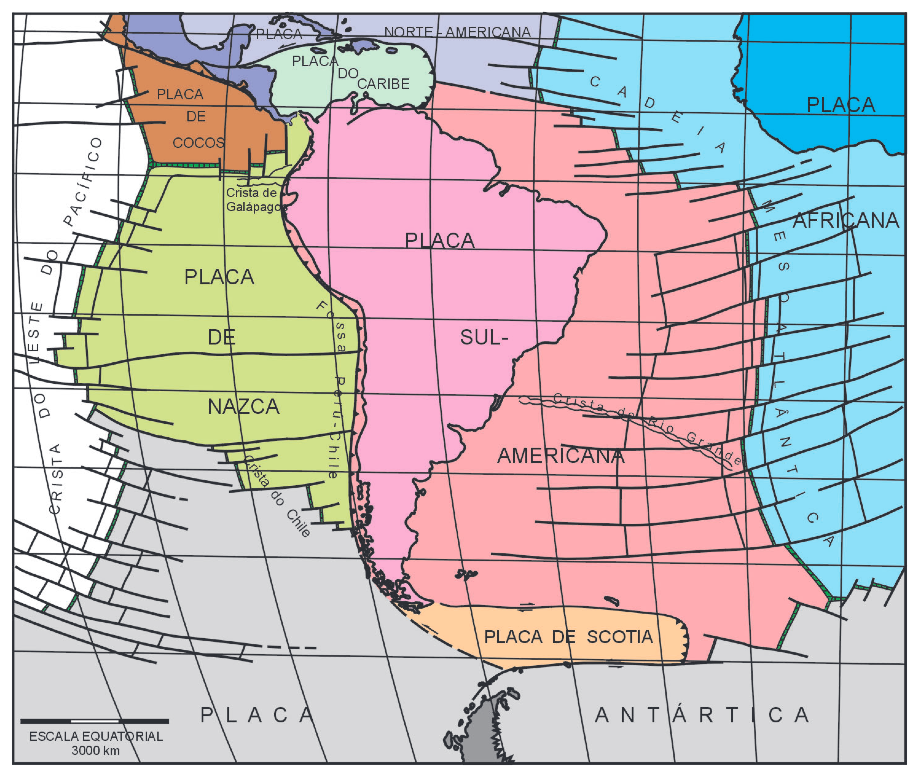
\includegraphics[width=.95\textwidth]{placas_sa} 
  \caption{Placa Sul-Americana em seu contexto global}
  \label{fig:sa_plate} 
\end{figure}


Na divisa com placa Africana à leste está a Dorsal Meso-Atlântica que é resultado
do processo de abertura dos oceanos e separação dos continentes. A abertura dos Atlântico na 
dorsal é responsável por um considerável esforço de compressão horizontal na placa Sul-Americana.

E há também a subducção da placa de Nazca sob a placa Sul-Americana, à oeste,
responsável, entre outros processos, pelo surgimento das Fossas Oceânicas e da
cordilheira dos Andes com suas altitudes e vulcanismo.

Olhando um pouco mais de perto para a parte continental da placa Sul-Americana
(figura \ref{fig:sa_tec}) é interessante destacar três grupos principais de rochas: 
(i) o Embasamento Pré-Cambriano, (ii) as Coberturas Fanerozóicas e (iii) a 
Cadeia Andina.

\begin{figure}[H]
  \centering
  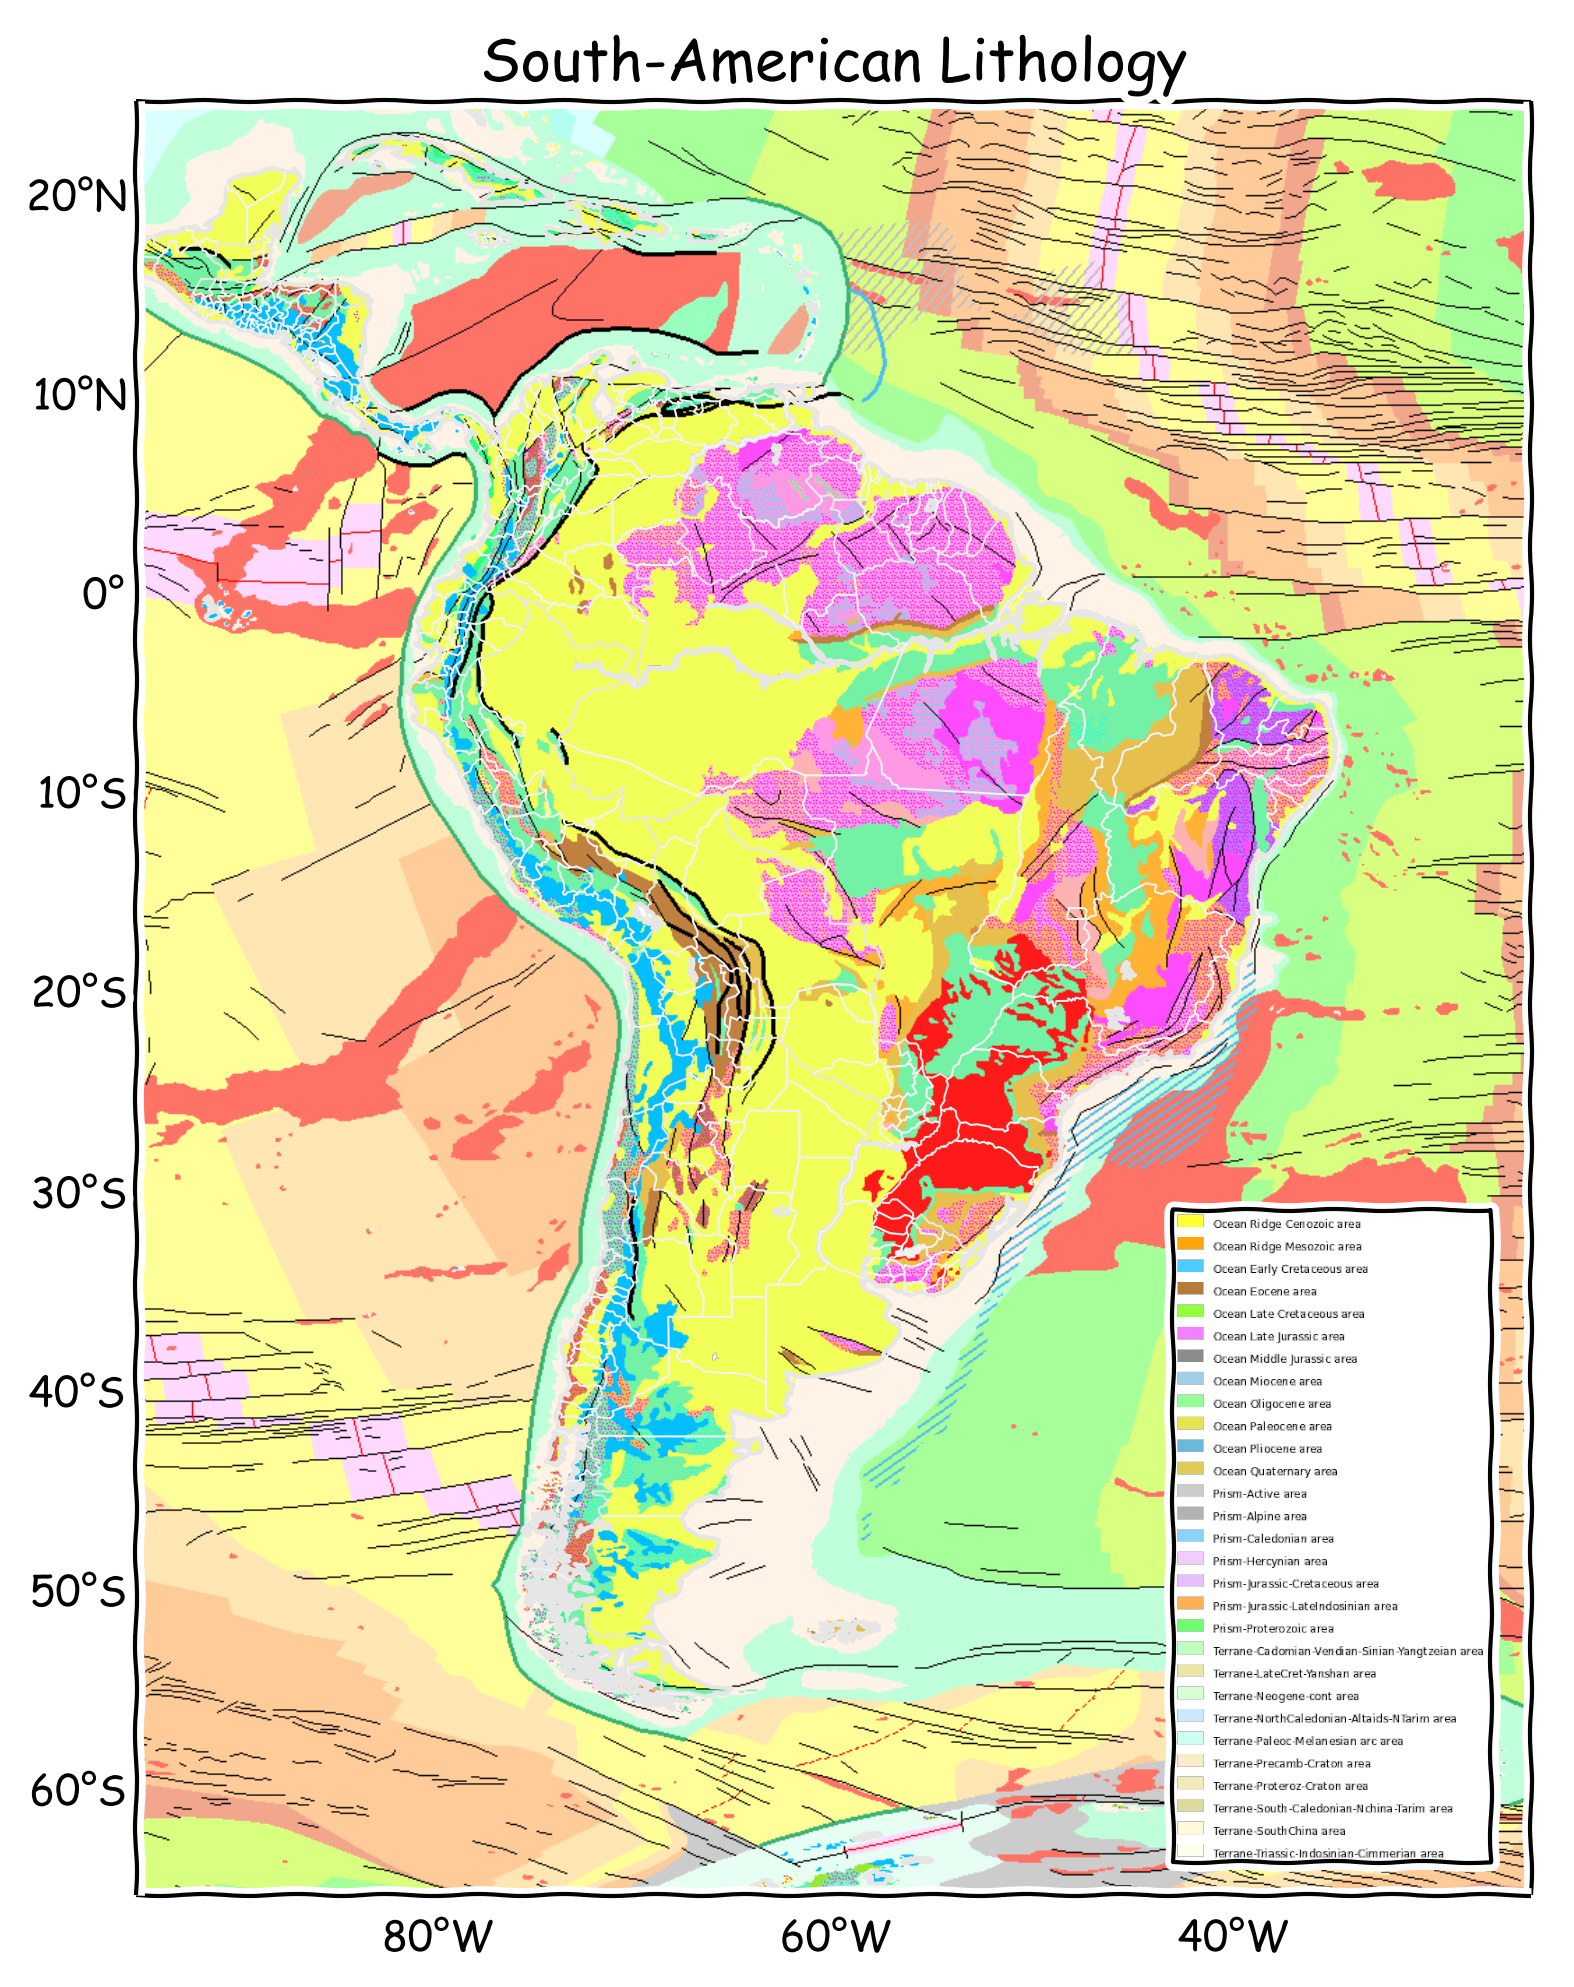
\includegraphics[width=.85\textwidth]{lithology_sa} 
  \caption{Mapa geológico da América do Sul. Fonte \url{http://onegeology.org}}
  \label{fig:sa_tec} 
\end{figure}

As rochas do embasamento pré-cambriano se originaram a mais de 500Ma. Por serem mais antigas
são mais estáveis. A cobertura Fanerozóica é resuldado da sedimentação ocorrida a menos de 250Ma. Formam as bacias
sedimentares. A Cadeia Andina com 30Ma é resultado da subducção e embora exponha rochas pré-cambrianas
em algumas partes é a parte mais ativa e interessante tectonicamente.


\subsubsection{Sismicidade Sul Americana}

A sismicidade Sul-Americana é marcada fortemente pela subducção à oeste e pela 
separação dos oceanos à leste. América Central, Caribe e a parte Antartica ao sul
são placas menores e seus movimentos merecem estudo de maior detalhe.

\begin{figure}[H]
  \centering
  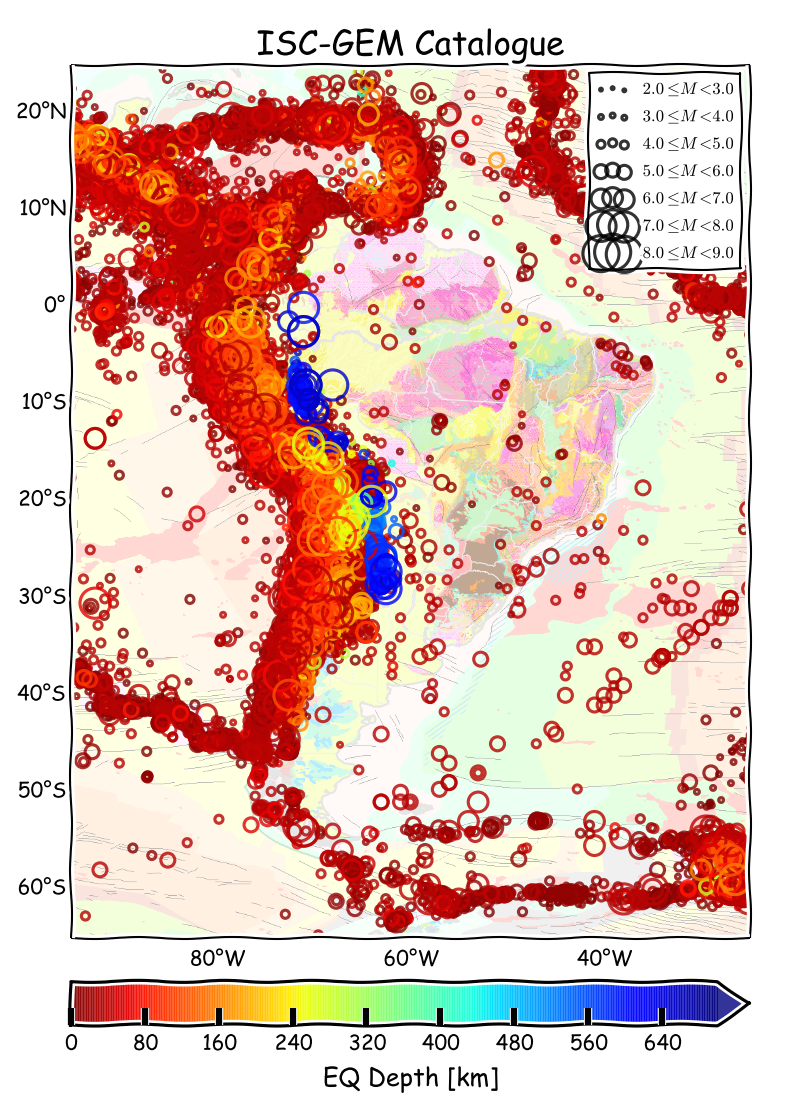
\includegraphics[width=.70\textwidth]{seismicity_sa} 
  \caption{Sismicidade da América do Sul, Catálogo \gls*{iscgem}. 
  		   Geologia: \gls*{cgmw} via OneGeology.
		   Sismos mais profundos foram registrados no interior da placa, inclusive sobre o Acre.
  		   }
  \label{fig:sa_seis} 
\end{figure}

A figura \ref{fig:sa_seis} apresenta a sismicidade da América do Sul pelo catálogo \gls{iscgem}
(seção \ref{sec:data_source}). É possivel notar claramente a subducção, ou seja, do mergulho, da placa de Nazca sob a placa
Sul-Americana. Fica mais claro quando se observa que os sismos com profundidade variando cerca de centenas de
quilômetros e que vão se tornando mais profundos para interior da placa Sul-Americana.

Isso acontece porque parte da quantidade de rocha fria, oceânica e continental, está afundando sob o manto
e lentamente se incorporando à ele. Mas ainda existem atrito, compressões e processos de ruptura nessas
profundidades e que ocorrem majoritariamente na interface entre essas placas pelo acúmulo de tensão e deslocamentos 
mínimos durante milhares de anos e que são liberados instantaneamente na ruptura. 
Esse processo é também o responsável pelo soerguimento da 
cordilheira dos Andes e de boa parte do vulcanismo na região. 

Sismos profundos, de 70 e 700km, geralmente provocam acelerações de baixa intensidade em seus epicentros 
devido à atenuação das ondas.

Também é latente a constatação da diferença de distribuição da sismicidade sul-americana nas bordas de placa e do
resto do continente como um todo. A maior parte do Brasil é praticamente inativa, não desprezível, no histórico
comparado.

%% ------------------------------------------------------------------------- %%
\section{Contexto Geológico e Tectônico Brasileiro}
\index{\gls{tectonic}!Brasil}
\label{sec:geotec_bras}

Tomando-se como referência 500Ma, destacam-se dois grandes grupos de rochas na figura \ref{fig:br_tec}
\citet{bizzi_2003} a seguir.

\begin{figure}[H]
  \centering
  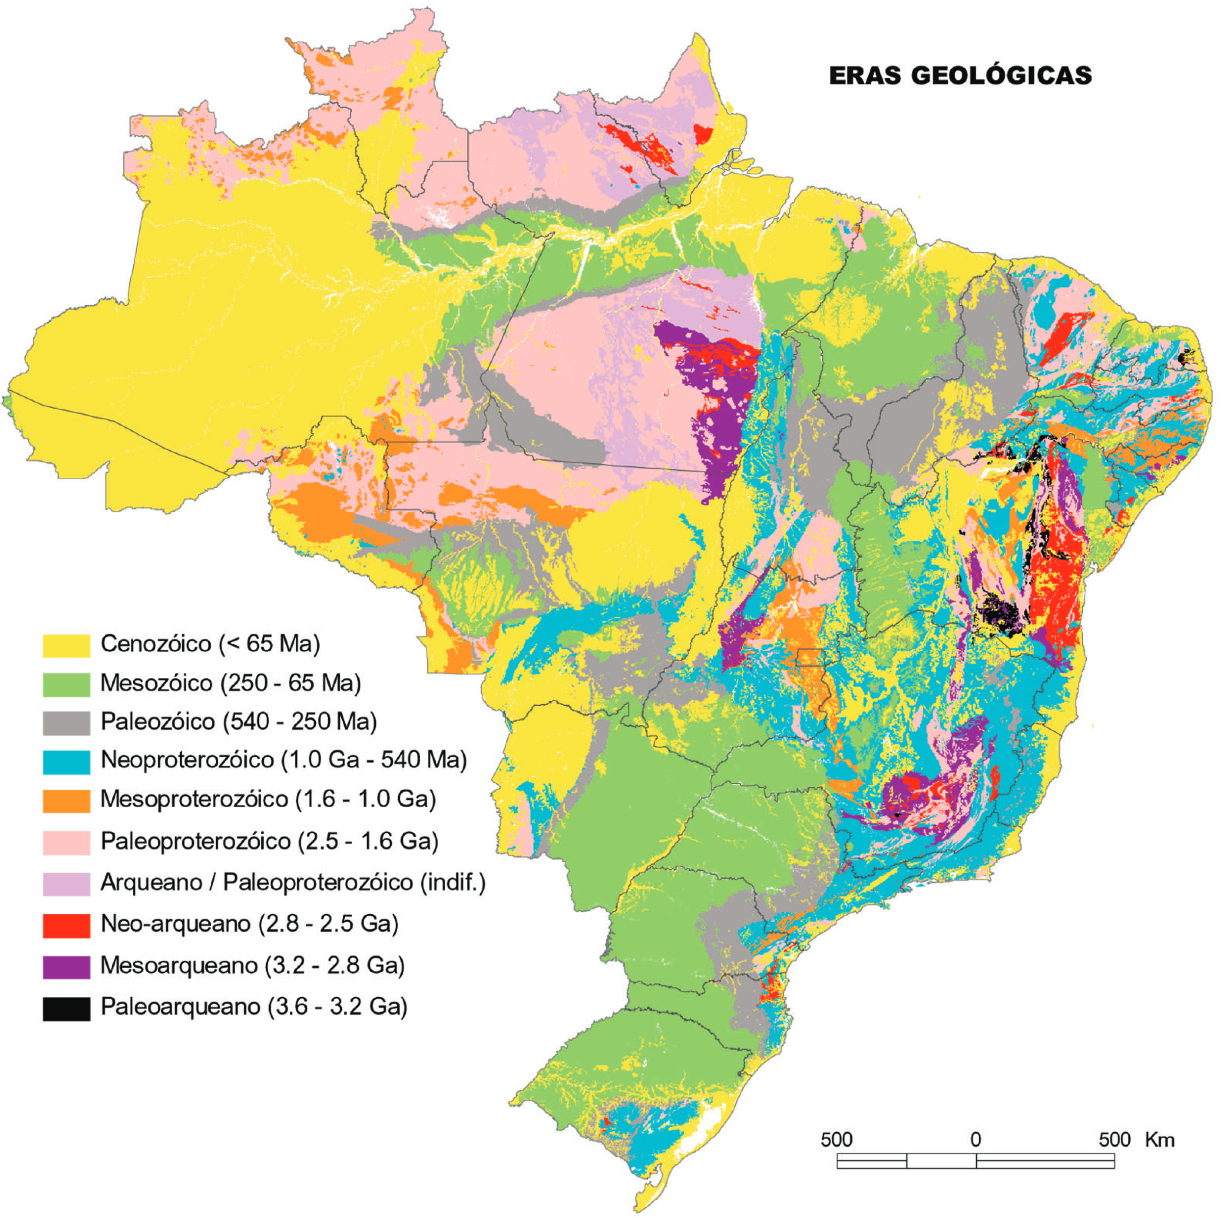
\includegraphics[width=.70\textwidth]{tectonico_brasil} 
  \caption{Mapa Geológico do Brasil em escala 1:1.000.000}.
  \label{fig:br_tec} 
\end{figure}

O embasamento, mais antigo, exposto sob a Amazônia e em porções menores e mais recentes também expostos 
no sudeste e nordeste, cedem espaço à um segundo grupo de rochas mais jovens, fruto da sedimentação e metamorfismos
mais recentes \citep{bizzi_2003}.


%% ------------------------------------------------------------------------- %%
\section{Sismicidade do Brasil}
\index{Sismicidade do Brasil}
\label{sec:sismicidade_brasil}

No Brasil não há terremotos. Não ao menos em quantidade proporcional a 10\% dos sismos sul-americanos.
Mesmo assim, ou por isso mesmo, a ocorrência de um sismo é ainda mais ameaçadora. Onde se espera, 
já se está preparado. Por outro lado onde nunca se espera é sempre uma surpresa.

É fato que o Brasil por estar numa área continental, mais no interior da placa \citep{talwani_2014} e geologia
com uma formação antiga e estável tem um número reduzido, não desprezível, de tremores. 
A figura \ref{fig:br_seis} mostra o detalhe da sismicidade brasileira com a litologia ao fundo.


\begin{figure}[H]
  \centering
  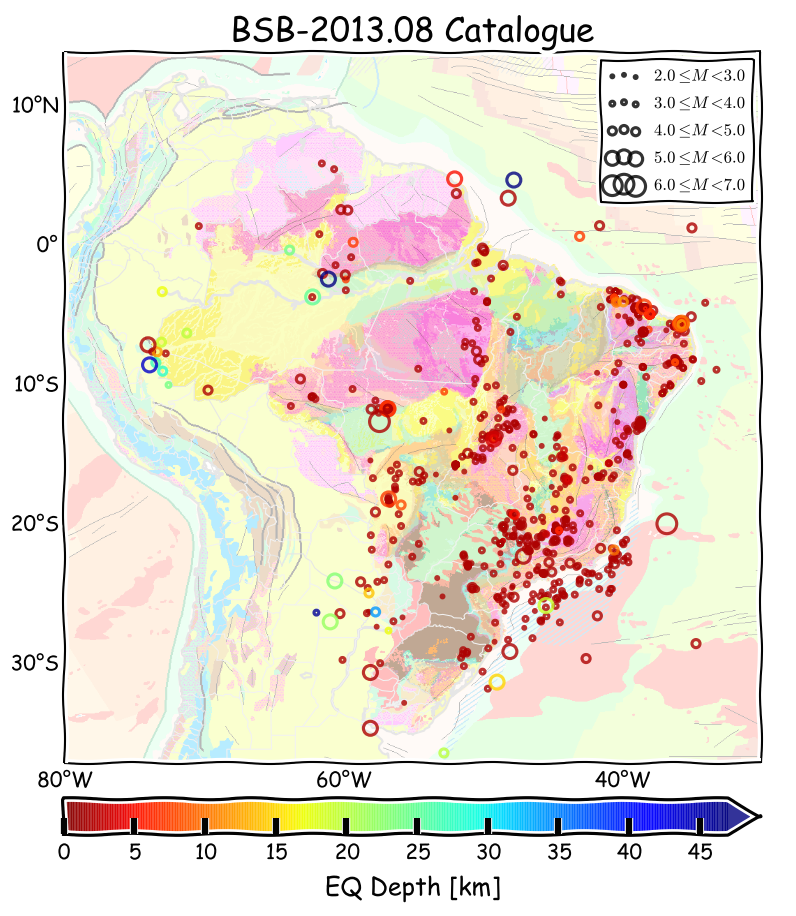
\includegraphics[width=.90\textwidth]{seismicity_br} 
  \caption{Sismicidade do Brasil. Catálogo \gls{bsb2013} (seção \ref{sec:data_source2}).}
  \label{fig:br_seis} 
\end{figure}

É importante notar que já houve registro de sismos com magnitudes pouco acima de 6,
e que sismos de magnitude acima de 4, rasos, em área urbana e em um continente estável,
com baixa atenuação das amplitudes das ondas sísmicas, podem ser danosos.


%% ------------------------------------------------------------------------- %%
\subsection{Sul, Sudeste e Litoral Leste}
\index{Sismicidade do Brasil!sul, sudeste e litoral leste}
\label{sec:z_se}

A sismicidade do sudeste e seu litoral possui características diferentes.
Enquanto no litoral, a principal sismiciade ocorre na área do talude continental
(porção dos fundos marinhos com declive muito pronunciado que fica entre a plataforma continental e
a margem continental e onde começam as planícies abissais), com destaque nessa sismicidade para um dos maiores sismos
que se tem registro no Brasil (figura \ref{fig:z_se}).

\begin{figure}[H]
  \centering
  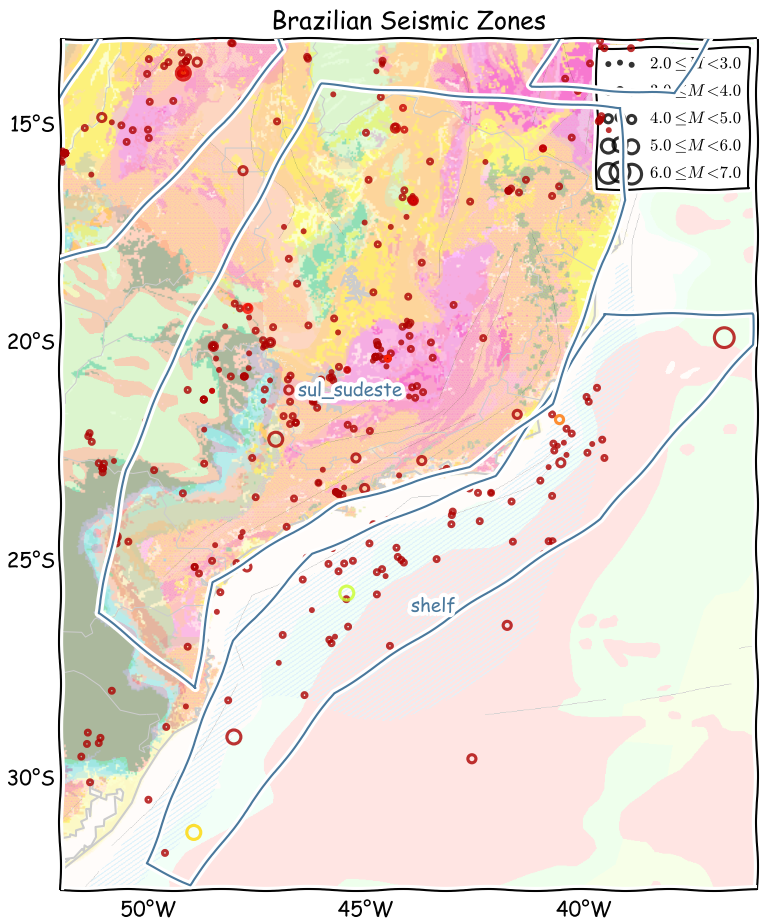
\includegraphics[width=0.6\textwidth]{z_se} 
  \caption{Zona sísmica do SE. \citet{dourado_2014}}
  \label{fig:z_se} 
\end{figure}

O continente é marcado por uma sismicidade difusa na área do cráton que se extende pelo norte de Minas
Gerais até quase o sul da Bahia e outra parte a nordeste da bacia do Paraná. 
Há também uma pequena sismicidade acompanhando a costa. Para maiores referencias, veja 
\citet{assumpcao_2004}.

É nessa região o único registro no Brasil de vítimas fatais decorrentes de tremores de terra, em Itacarambi, MG.

%% ------------------------------------------------------------------------- %%
\subsection{Centro-Norte}
\index{Sismicidade do Brasil!centro-norte}
\label{sec:z_cn}

É uma área com sismicidade peculiar. Na figura \ref{fig:z_cn}, de norte a sul, a sismicidade acompanha grosseiramente o
contato entre o cráton e parte da bacia do Parnaíba. O mesmo ocorre ambém no que seria a 
área central próxima à Chapada dos Veadeiros em uma outra formação cratônica.

\begin{figure}[H]
  \centering
  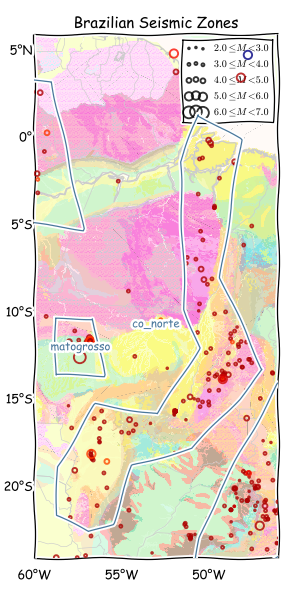
\includegraphics[width=0.45\textwidth]{z_co} 
  \caption{Zona sísmica do Centro-Norte. \citet{dourado_2014}}
  \label{fig:z_cn} 
\end{figure}

A última porção, ao sul, a sismicidade ocorre na área sedimentar da bacia do Pantanal.

%% ------------------------------------------------------------------------- %%
\subsection{Mato-Grosso}
\index{Sismicidade do Brasil!centro-norte}
\label{sec:z_mt}

A sismicidade do Mato-Grosso, mais precisamente de Porto-de-Gaúchos (\ref{fig:z_mt}), é emblemática para o Brasil.
Poderia ser considerada com características similares a Nova Madri, EUA.

\begin{figure}[H]
  \centering
  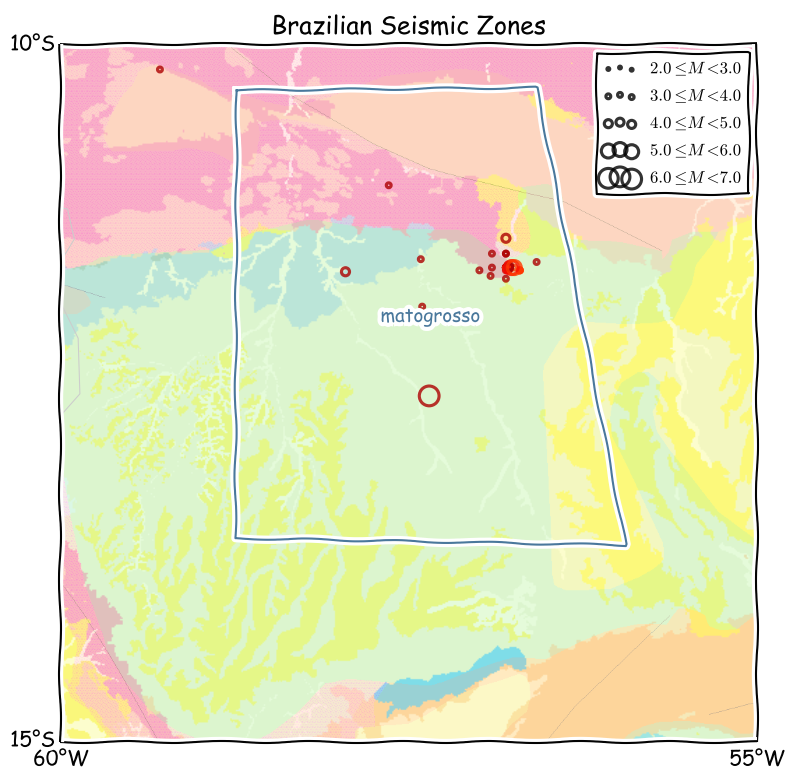
\includegraphics[width=0.45\textwidth]{z_mt} 
  \caption{Zona sísmica do Centro-Norte. \citet{dourado_2014}}
  \label{fig:z_mt} 
\end{figure}

A região sofreu um dos maiores sismos já registrados no Brasil, com magnitude pouco acima de 6.
Não há registros de falhas geológicas neo-tectônicas e mais complexa de ser explicada \citep{barros_2009}.

%% ------------------------------------------------------------------------- %%
\subsection{Extremo Oeste e Acre}
\index{Sismicidade do Brasil!extremo-oeste}
\label{sec:z_ac}

No extremo oeste do Brasil, na região do Acre, a sismicidade tem uma característica distinta das outras.
É possível reparar, na figura \ref{fig:z_ac}, primeiramente na quantidade de sismos, e em
seguida perceber a influência dos sismos sul americanos, desde os mais profundos aos intermediários
e relativamente rasos de 70km. 


\begin{figure}[H]
  \centering
  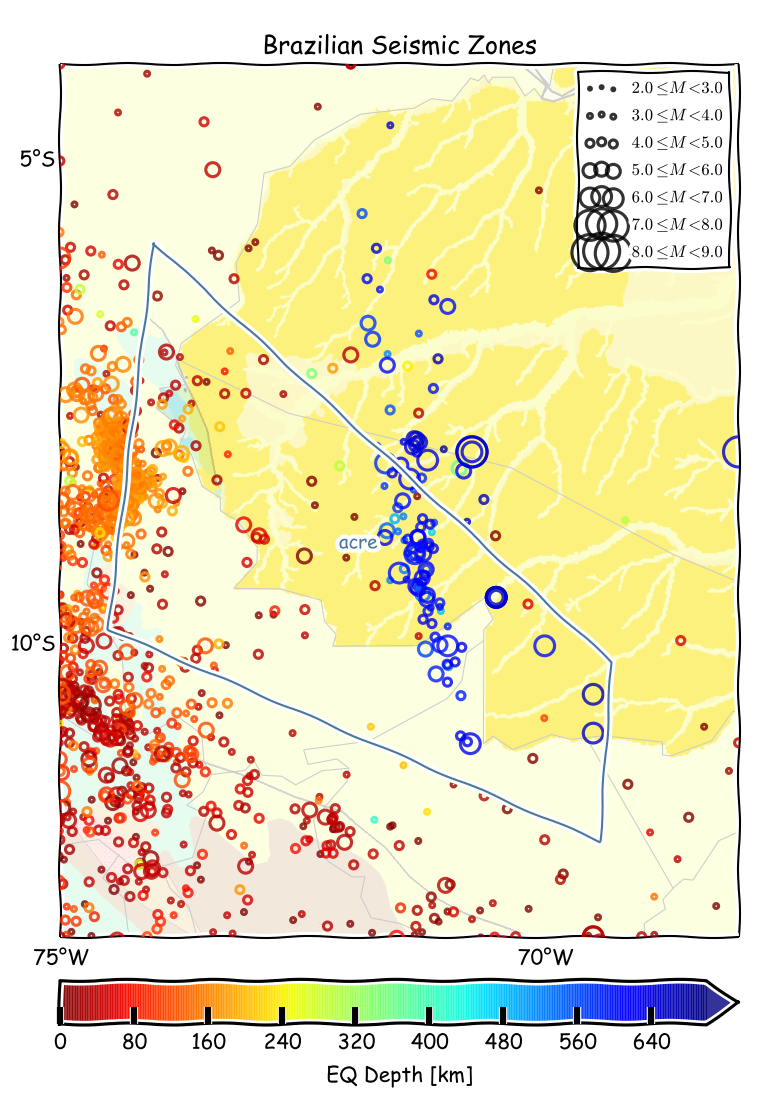
\includegraphics[width=0.5\textwidth]{z_ac} 
  \caption{Zona sísmica do Acre. \citet{dourado_2014}, Catálogo \gls*{iscgem}.}
  \label{fig:z_ac} 
\end{figure}

Note que a escala de profundidade da figura \ref{fig:z_ac} é diferente das demais que seguem a
mesma escala da figura \ref{fig:br_seis}.


%% ------------------------------------------------------------------------- %%
\subsection{Amazonas}
\index{Sismicidade do Brasil!Amazonas}
\label{sec:z_am}

É a região com menor quantidade de conhecimento e informação disponível.
Ainda assim, na figura \ref{fig:z_am} é possível observar a ocorrência de sismos
na direção norte-sul.

\begin{figure}[H]
  \centering
  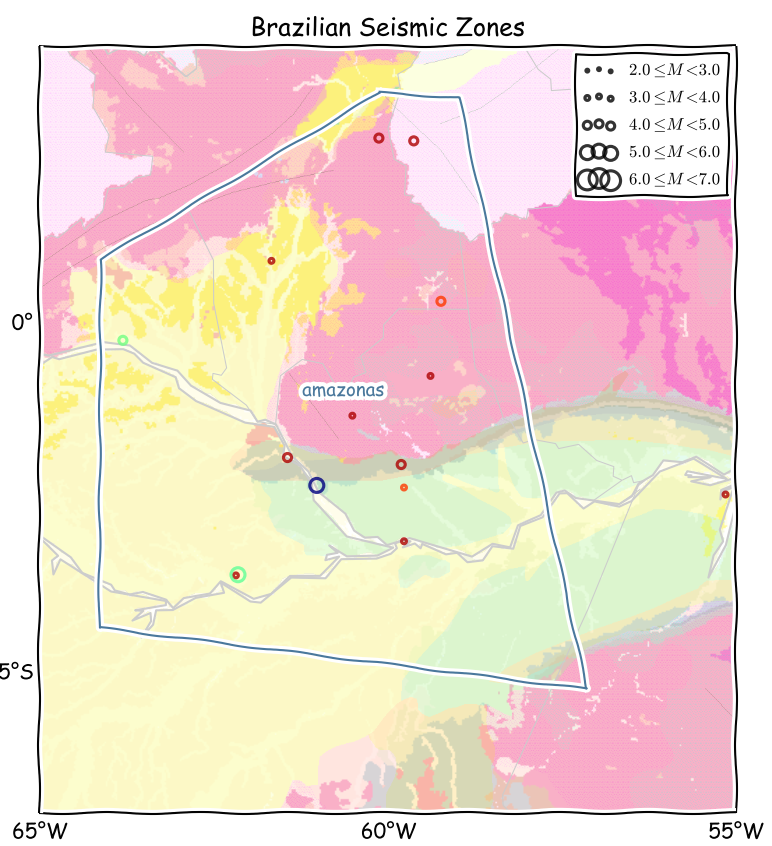
\includegraphics[width=0.5\textwidth]{z_am} 
  \caption{Zona sísmica de Manaus. \citet{dourado_2014}.}
  \label{fig:z_am} 
\end{figure}

O registro de um sismo de magnitude 5 determinada por dados macrossísmicos,
é o indício mais marcante na região.


%% ------------------------------------------------------------------------- %%
\subsection{Nordeste}
\index{Sismicidade do Brasil!nordeste}
\label{sec:z_ne}

A regisão nordeste brasileira é sismicamente a mais ativa (figura \ref{fig:z_ne}). 

\begin{figure}[H]
  \centering
  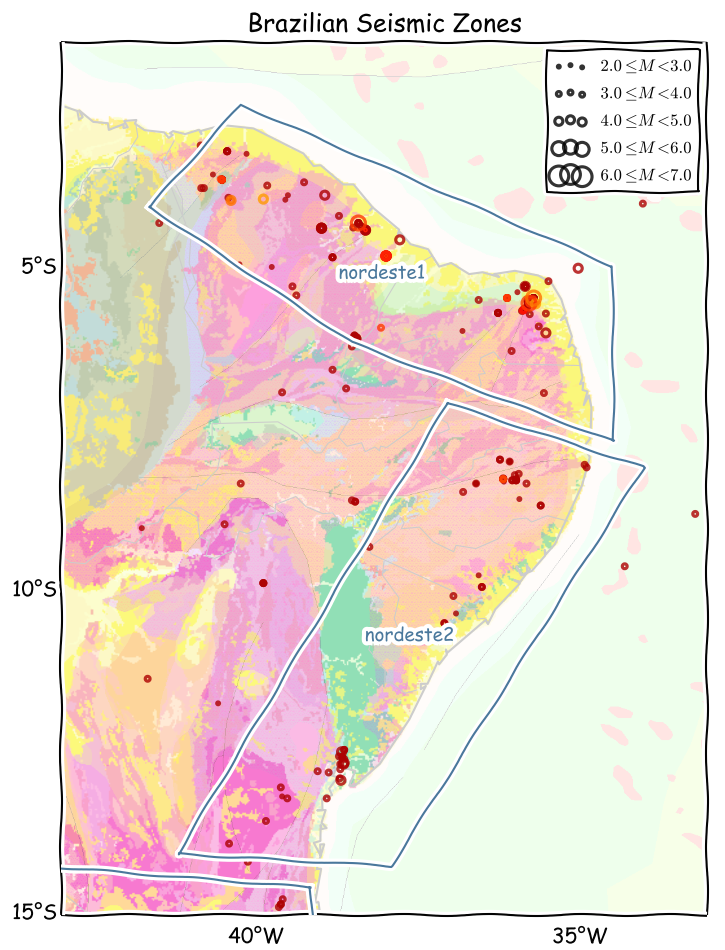
\includegraphics[width=0.6\textwidth]{z_ne} 
  \caption{Zona sísmica do NE. \citet{dourado_2014}}
  \label{fig:z_ne} 
\end{figure}

Destaca-se a sismicidade na região de João Câmara no Rio Grande do Norte,
com um enxame sísmico em meados da década de 1980 \citep{takeya_1989, bezerra_1998}. 
Além disso são bem conhecidas as atividades sísmicas na região de Sobral-CE,
na região de Pernambuco e um pouco mais ao sul já na Bahia.


